\documentclass[serif, xcolor=dvipsnames]{beamer}

\makeatletter

\documentclass[xcolor={usenames,svgnames,dvipsnames}]{beamer}
\usepackage[utf8]{inputenc}
\usepackage[T1]{fontenc}
\usepackage{graphicx}
\usepackage{grffile}
\usepackage{longtable}
\usepackage{wrapfig}
\usepackage{rotating}
\usepackage[normalem]{ulem}
\usepackage{amsmath}
\usepackage{textcomp}
\usepackage{amssymb}
\usepackage{capt-of}
\usepackage{hyperref}
\usepackage{color}
\usepackage{listings}
\usepackage{mathpazo}
\usepackage{gensymb}
\usepackage{amsmath}
\usepackage{chemarr}%flechas para reacciones químicas (SFER.tex)
\bibliographystyle{plain}
\AtBeginSubsection[]{\begin{frame}[plain]\tableofcontents[currentsubsection,sectionstyle=show/shaded,subsectionstyle=show/shaded/hide]\end{frame}}
\AtBeginSection[]{\begin{frame}[plain]\tableofcontents[currentsection,hideallsubsections]\end{frame}}
\usepackage[emulate=units]{siunitx}
\sisetup{fraction=nice, decimalsymbol=comma, retain-unity-mantissa = false}
\newunit{\wattpeak}{Wp}
\newunit{\watthour}{Wh}
\newunit{\amperehour}{Ah}
\usepackage{steinmetz}
\hypersetup{colorlinks=true, linkcolor=OliveGreen, urlcolor=Blue}
\renewcommand{\thefootnote}{\fnsymbol{footnote}}
\beamertemplatenavigationsymbolsempty
\setbeamertemplate{footline}[frame number]

\setbeamercolor{alerted text}{fg=Green!50!black} \setbeamerfont{alerted text}{series=\bfseries}
\usefonttheme{serif}
\setbeamercovered{transparent}
\setbeamertemplate{navigation symbols}{}
\usefonttheme{serif} 

\setbeamercolor{palette primary}{bg=OliveGreen,fg=white}
\setbeamercolor{palette secondary}{bg=OliveGreen,fg=white}
\setbeamercolor{palette tertiary}{bg=OliveGreen,fg=white}
\setbeamercolor{palette quaternary}{bg=OliveGreen,fg=white}
\setbeamercolor{structure}{fg=OliveGreen} % itemize, enumerate, etc
\setbeamercolor{section in toc}{fg=OliveGreen} % TOC sections

\usetheme[hideothersubsections]{Goettingen}

\usepackage{tikz}

\titlegraphic{
\includegraphics[width=2.5cm]{../figs/logoEOI.jpg}}
\addtobeamertemplate{frametitle}{}{%
\begin{tikzpicture}[remember picture,overlay]
\node[anchor=south east,yshift=2pt] at (current page.south east) {
\includegraphics[width=1.5cm]{../figs/logoEOI.jpg}};
\end{tikzpicture}}


\makeatother

\usepackage[spanish]{babel}
\addto\shorthandsspanish{\spanishdeactivate{~<>}}

\begin{document}

\title[\textsc{ESF: Diseño SFA}]{\textsc{Energía Solar Fotovoltaica:}\\
\textsc{Diseño de SFA}}


\author{\textsc{Oscar Perpiñán Lamigueiro}}

\date{}

\frame[plain]{\titlepage}

\AtBeginSection[]{
    \begin{frame}
        \frametitle{Índice}
        \tableofcontents[currentsection] 
    \end{frame} 

                  }

\selectlanguage{spanish}%

\section{Dimensionado del SFA}


\begin{frame}
\frametitle{Nomenclatura}
\begin{description}
\item [{Consumo:}] $L$
\item [{Probabilidad~de~pérdida~de~carga:}] relación entre la energía
que no puede suministrar el sistema fotovoltaico y la energía solicitada
por la carga durante todo el período de funcionamiento.\[
LLP=\frac{E_{def}}{L}\]

\end{description}

\end{frame}

\begin{frame}
\frametitle{Nomenclatura}
\begin{description}
\item [{Capacidad~del~generador:}] relación entre los valores medios
de la energía que puede producir el generador y la energía consumida
por la carga. \[
C_{A}=\frac{\eta_{G}\cdot A_{G}\cdot\overline{G_{d}}(\beta,\alpha)}{L}\]

\item [{Capacidad~de~acumulación:}] relación entre la capacidad útil
del acumulador y la energía consumida por la carga.\[
C_{s}=\frac{C_{U}}{L}=\frac{C_{B}\cdot PD_{max}}{L}\]

\end{description}

\end{frame}

\begin{frame}
\frametitle{Dimensionado}
\begin{block}
{}
\begin{itemize}
\item Diferentes valores de $(C_{A},\, C_{S})$ pueden conducir al mismo
valor de $LLP$.
\item Cuanto mayor es el sistema, mayor es la fiabilidad, pero mayor es
el coste.
\end{itemize}
\end{block}
{}
\begin{block}
{}

\textbf{La tarea de dimensionar un sistema fotovoltaico consiste en
encontrar la mejor solución de compromiso entre coste y fiabilidad.}

\end{block}

\end{frame}

\begin{frame}
\frametitle{Ciclado diario y estacional}
\begin{itemize}
\item El \textbf{ciclado diario }es la serie de cargas y descargas de la
batería que se producen durante un periodo diario. 

\begin{itemize}
\item $PD_{d}$, está relacionada con el consumo nocturno, $L_{n}$, y por
tanto exclusivamente con la capacidad de la batería: $PD_{d}=\frac{L_{n}}{C_{B}}$
\end{itemize}
\item El \textbf{ciclado estacional} es la serie de cargas y descargas que
se producen durante un periodo prolongado de duración variable 

\begin{itemize}
\item La duración, $D$, $PD_{e}$, están ligados al tamaño del generador,
al consumo diario (diurno y nocturno) y a la radiación disponible. 
\item La batería debe proporcionar la energía necesaria pero $PD_{e}<PD_{max}$. 
\end{itemize}
\end{itemize}

\end{frame}

\begin{frame}
\frametitle{Ciclado diario y estacional}
\begin{itemize}
\item La \textbf{combinación de $C_{A}$ alta y $C_{S}$ baja }conduce a
ciclados diarios con valores altos de $PD_{d}$ con ciclados estacionales
cortos. 

\begin{itemize}
\item Las descargas profundas y frecuentes asociadas al valor alto de $PD_{d}$
son perjudiciales para la batería, 
\item La corta longitud de los ciclados estacionales es beneficiosa. 
\item La estratificación será fácilmente compensable con sobrecargas controladas
aplicando el mantenimiento adecuado.
\end{itemize}
\end{itemize}

\end{frame}

\begin{frame}
\frametitle{Ciclado diario y estacional}
\begin{itemize}
\item La \textbf{combinación de $C_{A}$ baja y $C_{S}$ alta} conduce a
ciclados diarios con baja $PD_{d}$ y ciclados estacionales largos. 

\begin{itemize}
\item La baja $PD_{d}$ es beneficiosa para la batería, 
\item La longitud de los ciclados estacionales puede favorecer la sulfatación
y la estratificación. 
\item Dado el tamaño relativo del generador frente al acumulador, la frecuencia
de sobrecargas será baja y la estratificación no será tan fácilmente
compensada. 
\end{itemize}
\end{itemize}



\end{frame}

\begin{frame}
\frametitle{Métodos de dimensionado}
\begin{block}
{}
\begin{description}
\item [{Método~del~LLP:}] a partir de simulaciones o de curvas de isofiabilidad,
establece los valores de $C_{A}$ y $C_{S}$ para un consumo determinado.
\item [{Método~del~mes~peor:}] selecciona el tamaño de batería y generador
para abastecer el consumo durante el mes con peor relación entre radiación
y consumo (en los casos de consumo constante, el mes peor es aquel
de menor radiación). El tamaño de batería y generador se selecciona
en base a la experiencia acumulada según la zona geográfica y la aplicación
a abastecer.
\end{description}
\end{block}

\end{frame}

\begin{frame}
\frametitle{Método del LLP}
\begin{block}
{Suposiciones}
\begin{itemize}
\item El consumo es constante a lo largo del año
\item Todo el consumo ocurre por la noche
\item Los componentes del sistema FV no tienen pérdidas (incluidas dentro
de $C_{A}$ y $C_{S}$) y lineales.
\end{itemize}
\end{block}

\end{frame}

\begin{frame}
\frametitle{Método del LLP}
\begin{block}
{Simulación del sistema}

\[
SOC_{j}=min[SOC_{j-1}+\frac{C_{A}\cdot G_{d,j}}{C_{s}\cdot\overline{G_{d}}}-\frac{1}{C_{s}};1]\]


\[
E_{def}=max\{\frac{1}{C_{s}}-SOC_{j};0\}\]


Se considera que hay deficit de energía cuando la almacenada al final
del día ($SOC_{j}\cdot C_{S}\cdot L$) no es suficiente para abastecer
el consumo diario ($L$). Es decir, \[
SOC_{j}\cdot C_{s}\cdot L<L\Rightarrow\frac{1}{C_{s}}-SOC_{j}>0\]


\[
LLP=\frac{\sum_{1}^{N}E_{def}}{N\cdot L}\]


\end{block}

\end{frame}

\begin{frame}[plain]
\frametitle{Método de LLP}

\begin{center}
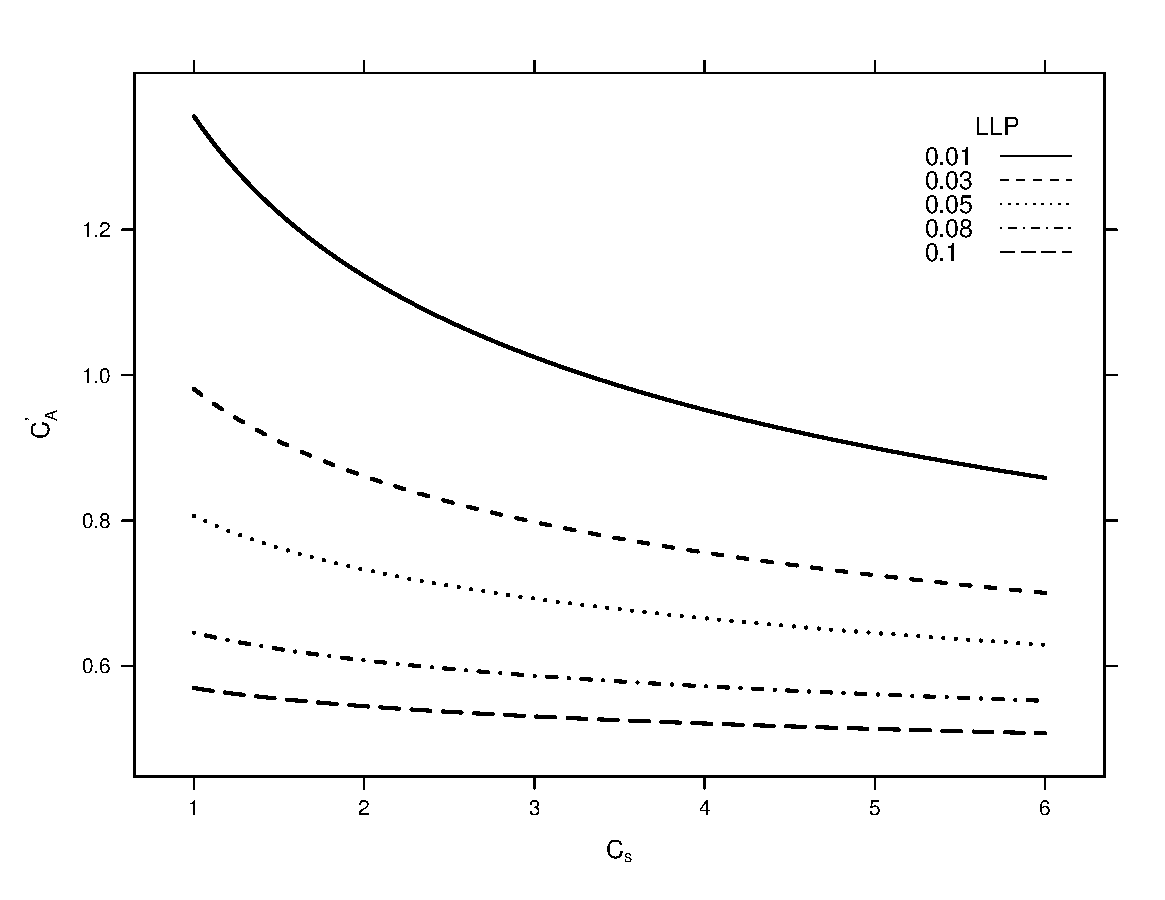
\includegraphics[scale=0.5]{../Figuras/CurvasLLP}
\par\end{center}


\end{frame}

\begin{frame}[plain]
\frametitle{Relación entre $C_{A}^{'}$ y LLP}


\framesubtitle{$C_{s}=3$}

\begin{center}
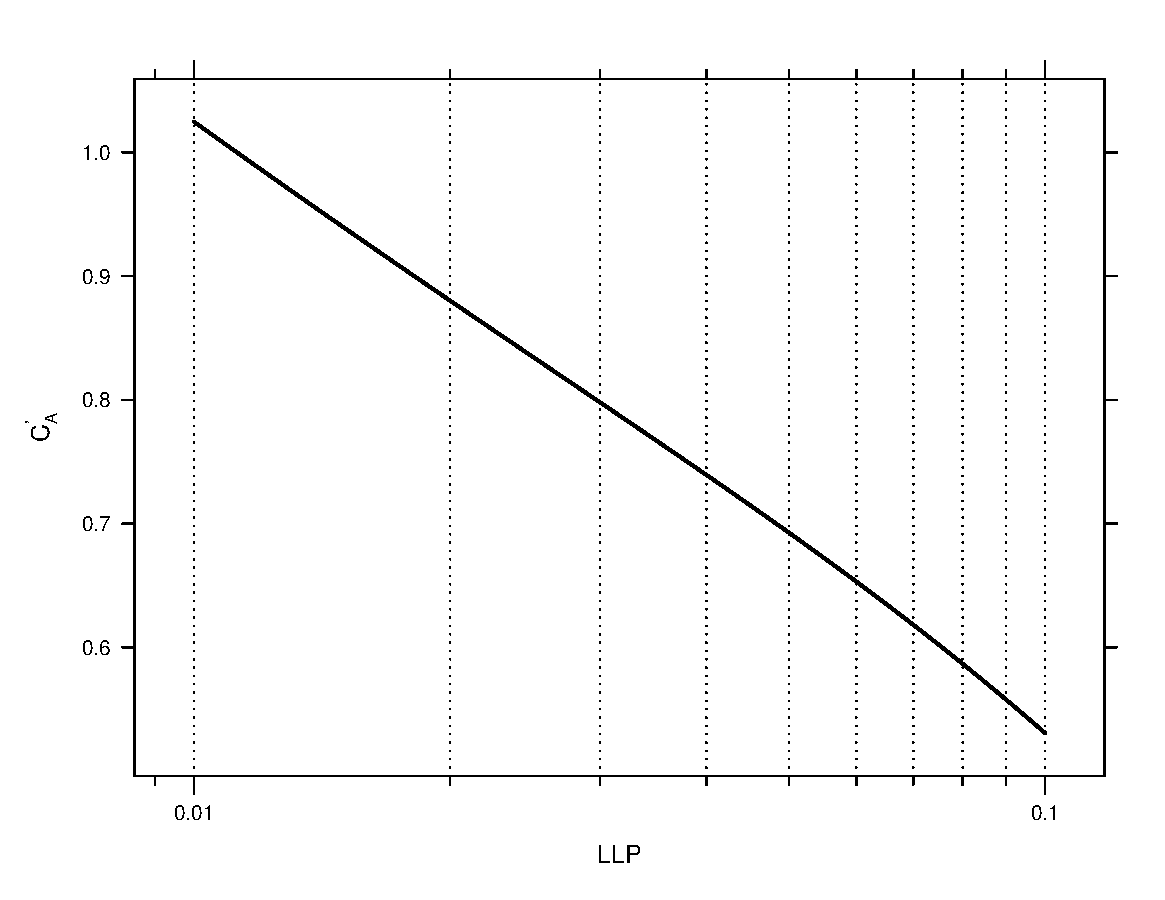
\includegraphics[scale=0.5]{../Figuras/CurvasLLP_Cs3}
\par\end{center}


\end{frame}

\begin{frame}
\frametitle{Método del LLP}
\begin{block}
{}

Es posible ajustar las curvas isofiables a una ecuación analítica:\begin{eqnarray*}
C_{A}^{'} & = & f\cdot C_{s}^{-u}\end{eqnarray*}


donde $f$ y $u$ son dos parámetros sin significado físico, dependientes
del lugar y del LLP deseado. Para su determinación es necesario realizar
varias simulaciones previas.

\end{block}

\end{frame}

\begin{frame}
\frametitle{Método de LLP}
\begin{itemize}
\item Este proceso de cálculo se apoya en series de valores de radiación
solar que reproducen el comportamiento estadístico de la irradiación. 
\item Predicción del comportamiento del sistema limitada por la incertidumbre
asociada. 
\item Los ejercicios de cálculo para probabilidades de pérdida de carga
inferiores a $LLP=\num{1e-2}$ carecen de utilidad.\end{itemize}
\begin{block}
{}

{}``{[}...{]} los modelos de simulación muy exactos pueden proporcionar
números también muy exactos, pero ello no significa que se traduzcan
automáticamente en predicciones también muy exactas.''

\end{block}

\end{frame}

\begin{frame}
\frametitle{Método del mes peor}
\begin{block}
{Valores según el UTS for SHS}
\begin{description}
\item [{Electrificación~rural:}] $C_{A}=1.1$ y $3\leq C_{S}\leq5$
\item [{Aplicaciones~profesionales:}] $1.2\leq C_{A}\leq1.3$ y $5\leq C_{S}\leq8$
\end{description}
\end{block}
{}
\begin{block}
{Valores de común uso en España}

\begin{center}
\begin{tabular}{ccccc}
\toprule 
 & \multicolumn{4}{c}{Aplicación}\tabularnewline
\cmidrule{2-5} 
 & \multicolumn{2}{c}{Doméstica} & \multicolumn{2}{c}{Profesional}\tabularnewline
\midrule
\midrule 
Zona & $C_{A}$ & $C_{S}$ & $C_{A}$ & $C_{S}$\tabularnewline
\midrule 
Norte de España & 1.2 & 5 & 1.3 & 8\tabularnewline
\midrule 
Sur de España & 1.1 & 4 & 1.2 & 6\tabularnewline
\bottomrule
\end{tabular}
\par\end{center}

\end{block}

\end{frame}

\begin{frame}
\frametitle{Configuración de generador y batería}

Una vez elegidos los valores de $C_{A}$ y $C_{S}$, se deben configurar
el generador y batería de acuerdo a las tensiones de trabajo. En general,
la batería impone la tensión de trabajo (no hay buscador de MPP).
Supondremos $V_{mpp}\simeq V_{b}$

\begin{eqnarray*}
L & = & V_{b}\cdot Q_{L}\\
\eta_{G}\cdot A_{G}\cdot G_{stc} & = & I_{g}^{*}\cdot V_{b}\end{eqnarray*}



\end{frame}

\begin{frame}
\frametitle{Configuración de generador y batería}

y por tanto:\begin{eqnarray*}
I_{g}^{*} & = & \frac{C_{A}\cdot Q_{L}\cdot G_{stc}}{\overline{G_{d}}(\beta,\alpha)}\\
Q_{B} & = & C_{S}\cdot Q_{L}\end{eqnarray*}


siendo $Q_{L}$ la carga a satisfacer en amperios-hora, y $Q_{B}$
la capacidad útil de la batería en amperios-hora.


\end{frame}

\begin{frame}
\frametitle{Inclinación del generador}
\begin{itemize}
\item Para instalaciones con \textbf{consumos constantes o similares a lo
largo del año}, se busca maximizar la radiación en los meses de menor
insolación\[
\beta=|\phi|+10^{\circ}\]

\item Para instalaciones con \textbf{consumo menor en meses de baja radiación}
se busca maximizar radiación en equinoccios.\[
\beta=|\phi|\]

\item Para instalaciones con \textbf{uso predominante en verano} (hemisferio
Norte) conviene emplear un ángulo inferior a la latitud.\[
\beta=|\phi|-10^{\circ}\]

\item En general, la inclinación \textbf{debe superar} los $15^{\circ}$.
\end{itemize}

\end{frame}

\section{Estimación del consumo}


\begin{frame}
\frametitle{Cálculo del consumo}

\[
L_{T}=\frac{L_{dc}}{\eta_{r}}+\frac{L_{ac}}{\eta_{inv}}\]


\[
L=\frac{L_{T}}{\eta_{bat}\cdot\eta_{c}}\]


\begin{center}
Como valores orientativos pueden utilizarse
\par\end{center}

\begin{center}
$\eta_{inv}=0.9$, $\eta_{r}=0.95$, $\eta_{bat}=0.85$ y $\eta_{c}=0.98$.
\par\end{center}


\end{frame}

\begin{frame}[plain]
\frametitle{Distribución del consumo}

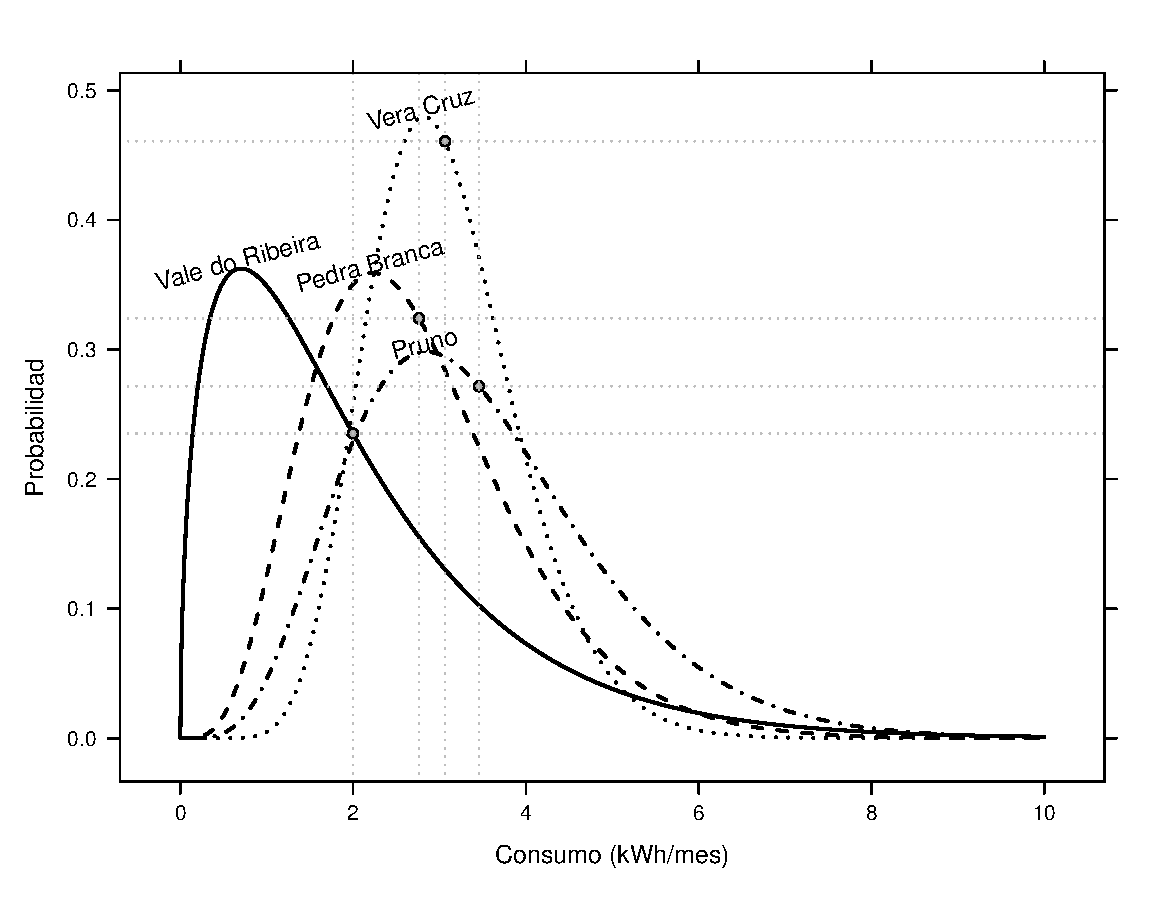
\includegraphics[scale=0.55]{../Figuras/ConsumoGamma}


\end{frame}

\begin{frame}[plain]
\frametitle{Relación entre el consumo y la fiabilidad}

\begin{center}
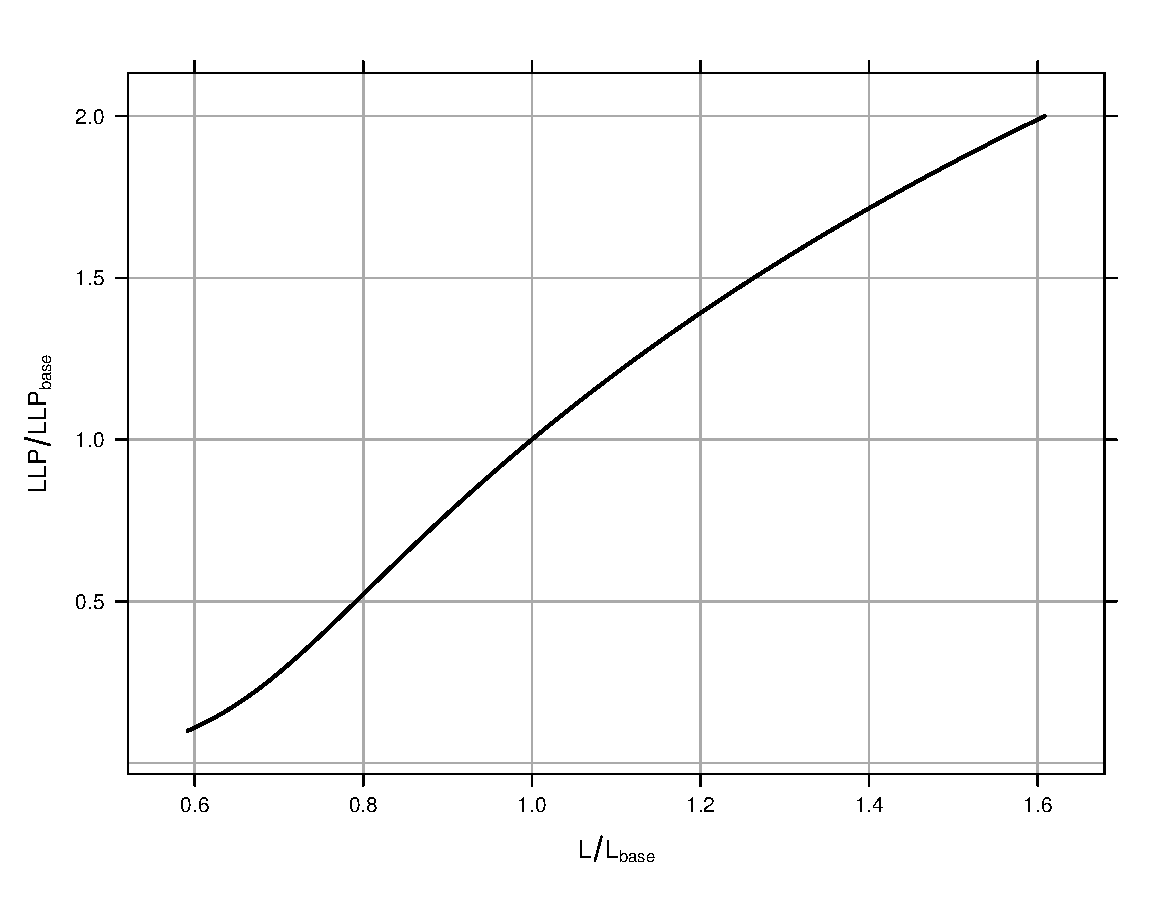
\includegraphics[scale=0.55]{../Figuras/ConsumoLLP}
\par\end{center}


\end{frame}

\begin{frame}
\frametitle{Escenarios de consumo}

\begin{tabular}{>{\centering}p{2cm}>{\centering}p{4cm}>{\centering}p{2cm}}
\toprule 
Aplicación & Hipótesis de consumo & Criterio de dimensionado\tabularnewline
\midrule
\midrule 
SHS1 & \begin{itemize}
\item Iluminación
\item Radio 
\item TV b/n, 
\item Sin frigorífico: 
\item 120 Wh/dia
\end{itemize}
 & \begin{eqnarray*}
C_{A} & = & 1.1\\
3\leq & C_{s} & \leq5\end{eqnarray*}
\tabularnewline
\bottomrule
\end{tabular}


\end{frame}

\begin{frame}
\frametitle{Escenarios de consumo}

\begin{tabular}{>{\centering}p{2cm}>{\centering}p{4cm}>{\centering}p{2cm}}
\toprule 
Aplicación & Hipótesis de consumo & Criterio de dimensionado\tabularnewline
\midrule
\midrule 
SHS2 & \begin{itemize}
\item Iluminación
\item Radio
\item TV color
\item Sin frigorífico
\item 250 Wh/dia
\end{itemize}
 & \begin{eqnarray*}
C_{A} & = & 1.1\\
3\leq & C_{s} & \leq5\end{eqnarray*}
\tabularnewline
\bottomrule
\end{tabular}


\end{frame}

\begin{frame}
\frametitle{Escenarios de consumo}

\begin{tabular}{>{\centering}p{2cm}>{\centering}p{4cm}>{\centering}p{2cm}}
\toprule 
Aplicación & Hipótesis de consumo & Criterio de dimensionado\tabularnewline
\midrule
\midrule 
SHS3 & \begin{itemize}
\item Iluminación
\item radio
\item TV color
\item Con frigorífico eficiente
\item 1000 Wh/dia
\end{itemize}
 & \begin{eqnarray*}
C_{A} & = & 1.1\\
C_{S} & = & 5\end{eqnarray*}
\tabularnewline
\bottomrule
\end{tabular}


\end{frame}

\begin{frame}
\frametitle{Escenarios de consumo}

\begin{tabular}{>{\centering}p{2cm}>{\centering}p{4cm}>{\centering}p{2cm}}
\toprule 
Aplicación & Hipótesis de consumo & Criterio de dimensionado\tabularnewline
\midrule
\midrule 
Centrales & \begin{itemize}
\item Todo AC 
\item 500 Wh/dia por vivienda. 
\end{itemize}
 & \begin{eqnarray*}
C_{A} & = & 1.1\\
C_{S} & = & 5\end{eqnarray*}
\tabularnewline
\bottomrule
\end{tabular}


\end{frame}


\end{document}
